%! TeX program = lualatex
%----------------------------------------------------------------------------------------
%    PACKAGES AND THEMES
%----------------------------------------------------------------------------------------

\documentclass[aspectratio=169,xcolor=dvipsnames,10pt]{beamer}
\usetheme{SimplePlus}

\usepackage{hyperref}
\usepackage{graphicx} % Allows including images
\usepackage{booktabs} % Allows the use of \toprule, \midrule and \bottomrule in tables
\usepackage{bbm}
\usepackage{bm}
\usepackage{mathtools}
\usepackage{amsthm}
\usepackage{tikz-cd}
\usepackage{listings}

%%%%%%% JULIA %%%%%%%%%%
\usepackage{fontspec}

\newfontfamily\JuliaMono{JuliaMono}[
	UprightFont = *-Regular,
	BoldFont = *-Bold,
	Path =/Users/davibarreira/Library/Fonts/,
	Extension = .ttf]
\newfontface\JuliaMonoRegular{JuliaMono-Regular}
\newfontface\JuliaMonoBold{JuliaMono-Bold}
% \setmonofont{JuliaMono-Light}[Contextuals=Alternate]


\input{julia_listings}
\input{julia_listings_unicode}

\lstdefinelanguage{JuliaLocal}{
    language = Julia, % inherit Julia lang. to add keywords
}
% \newcommand{\pc}[1]{\lstinline[style=julia]{#1}}
\newcommand{\pc}[1]{\lstinline[style=juliasmall]{#1}}
\newcommand{\pcsmall}[1]{\lstinline[style=juliasmall]{#1}}
\renewcommand{\lstlistingname}{Code}
%%%%%%%%%%%%%%%%%%%%%%%%


\theoremstyle{definition}
\newtheorem{proposition}{Proposition}

\usepackage[square,numbers]{natbib}
\newcommand*{\QEDA}{\hfill\ensuremath{\blacksquare}}%
\newcommand*{\QEDB}{\hfill\ensuremath{\square}}%

%----------------------------------------------------------------------------------------
%    TITLE PAGE
%----------------------------------------------------------------------------------------

\title{Data Visualization From a Category Theory Perspective}
\subtitle{}

\author{Davi Sales Barreira, Asla Medeiros e Sá}

\institute
{
    FGV - EMAp, IMPATech
}
\date{\today} % Date, can be changed to a custom date

%----------------------------------------------------------------------------------------
%    PRESENTATION SLIDES
%----------------------------------------------------------------------------------------
\setbeamertemplate{blocks}[default]
\setbeamercolor{block title}{fg=white, bg=RoyalBlue}
\setbeamercolor{block body}{fg=black, bg=white}

\begin{document}

\begin{frame}
    % Print the title page as the first slide
    \titlepage
\end{frame}

%------------------------------------------------
\begin{frame}{Table of contents}
    \begin{enumerate}
        \item Vizagrams Hands-on
        \item Category Theory behind Vizagrams
    \end{enumerate}
\end{frame}

\begin{frame}{Introduction}
    \centering
    Balance expressiveness and abstraction in data visualization frameworks.
    \\[1em]
    
\includegraphics[width=0.8\textwidth]{./figures/expressiveness.pdf}
\end{frame}

\begin{frame}{Introduction}
    \centering
    Visualization grammars often come short in terms of expressiveness, e.g., composite visualizations and visualizations with custom marks.
    \\[1em]
    \includegraphics[width=\textwidth]{figs/compvis.png}
\end{frame}

\begin{frame}{Introduction}
    \centering
    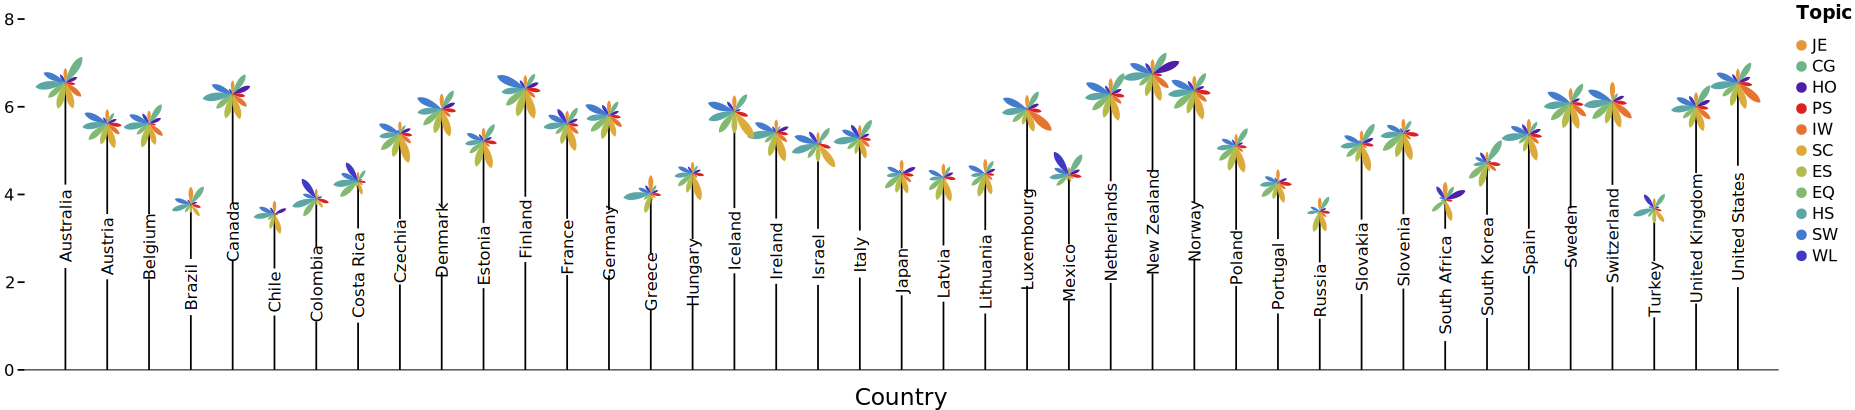
\includegraphics[width=\textwidth]{./figs/moritz.pdf}
\end{frame}

\begin{frame}{Introduction}
    \centering
    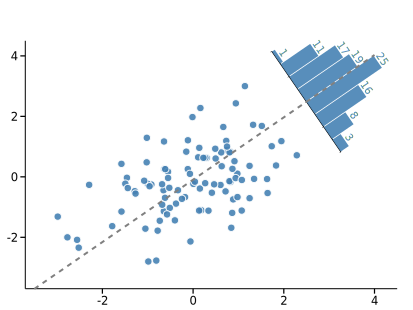
\includegraphics[width=0.55\textwidth]{./figs/pca.pdf}
\end{frame}

\begin{frame}{Introduction - Objective and Hypotheses}
    \textbf{Main Objective:} Develop a data visualization framework that extends the expressiveness of visualization grammars while preserving a high level of abstraction.
    \\[1em]
    \textbf{Hypothesis 1 (Cause):} Limitations in expressiveness are due to a lack of integration between graphic specification and assembly.
    \\[1em]
    \textbf{Hypothesis 2 (Solution):} Integration of diagramming and graphic specification via a unified constructive framework.
    \\[1em]
    \textbf{Formalization Tool:} Category Theory.
\end{frame}

\begin{frame}{Introduction - Overview}
    \centering
    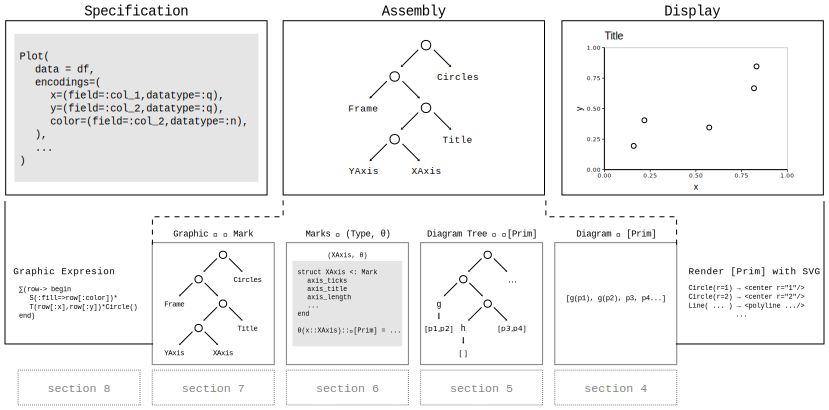
\includegraphics[width=0.9\textwidth]{figs/pipe.pdf}
\end{frame}

\begin{frame}{Data Visualization + Category Theory: Diagrams as Monoids}
    The basic building block for any diagram is the primitive.
    A primitive is any geometry that can be drawn and manipulated via geometric or stylistic transformations.
    \\[1em]
    \begin{center}
    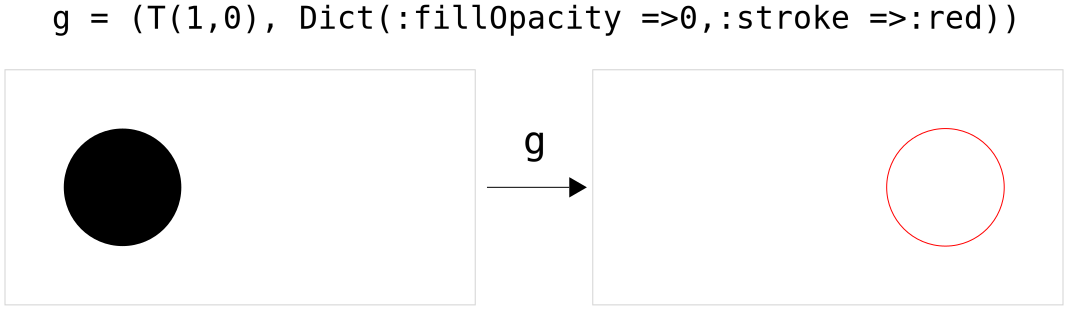
\includegraphics[width=0.7\textwidth]{figs/primitivetransformation.pdf}
    \end{center}
\end{frame}

\begin{frame}[fragile]{Data Visualization + Category Theory: Diagrams as Monoids}
    A diagram can be defined as an ordered list of primitives.
    $( [\text{Prim}] , +, [\ ] )$ can be interpreted as a monoid.
\begin{lstlisting}[language=JuliaLocal, style=julia, texcl=true, escapeinside={(@}{@)}]
abstract type Prim end
struct Circle <: Prim
  radius::Real
  center::Tuple{Real, Real}
end
+(d1::Vector{Prim}, d2::Vector{Prim}) = vcat(d1,d2)
\end{lstlisting}
\end{frame}

\begin{frame}[fragile]{Data Visualization + Category Theory: Diagrams as Monoids}

    Diagrams are drawn by rendering the list of primitives on top of each other.
    \begin{center}
        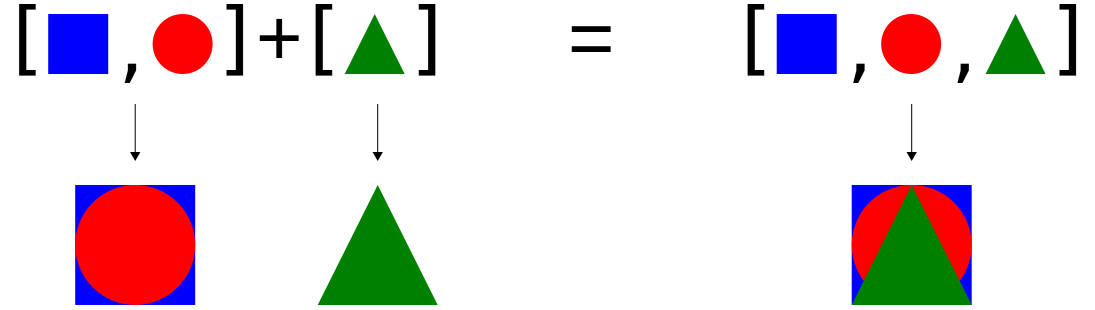
\includegraphics[width=0.7\textwidth]{./figs/simplediagram.pdf}
    \end{center}
\end{frame}

\begin{frame}[fragile]{Data Visualization + Category Theory: Diagrams as Monoids}

  We can apply transformations to diagrams by applying the
  transformations to each primitive in the list.
    \begin{center}
        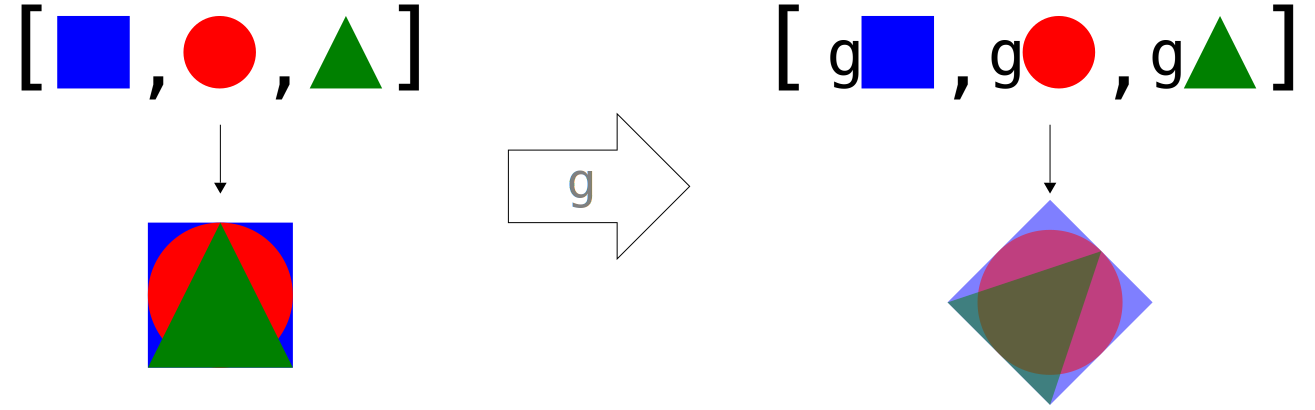
\includegraphics[width=0.7\textwidth]{./figs/diagramtransformation.pdf}
    \end{center}
\end{frame}

\begin{frame}[fragile]{Data Visualization + Category Theory}
    \centering
    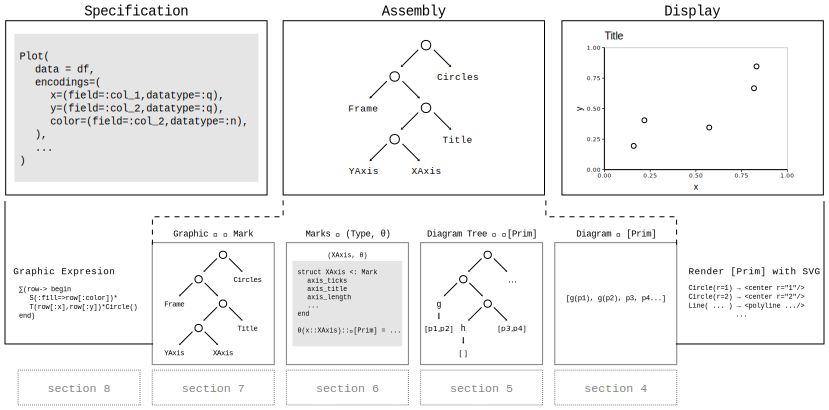
\includegraphics[width=0.9\textwidth]{figs/pipe.pdf}
\end{frame}

\begin{frame}[fragile]{Data Visualization + Category Theory: Free Monads}

  Let us improve our representation using expression trees.
  To do this, first we define a functor $F$ that encodes
  diagram composition (i.e. $+$) and diagram transformations.
\begin{lstlisting}[language=JuliaLocal, style=julia, texcl=true, escapeinside={(@}{@)}]
@data F{a} begin
Comp(::a, ::a)
Act(::H, ::a)
end
fmap(f::Function, x::Comp) = Comp(f(x._1),f(x._2))
fmap(f::Function, x::Act) = Act(x._1,f(x._2))
\end{lstlisting}

\end{frame}

\begin{frame}[fragile]{Data Visualization + Category Theory: Free Monads}

  Using our functor $F$, we can define a free monad over
  such functor, i.e $\mathbb T := \text{Free} F$. Thus,
  $(\mathbb T, \eta, \mu)$ is our monad, where $\mathbb T$ is a parametric type
  representing trees with $F$ as possible operations.

  To ease the process of expressing trees, we overload
  the $+$ and the $*$ operators to represent composition
  and transformation application respectively.

  \begin{figure}
    \begin{center}
        
\includegraphics[width=0.6\textwidth]{./figs/composetrees.pdf}
    \end{center}
  \end{figure}
  
\end{frame}

\begin{frame}[fragile]{Data Visualization + Category Theory: Free Monads}

    A diagram tree is a value of type $\mathbb T$ [Prim]. For this representation to
  be useful, we must be able to flatten it, i.e.
  we must define a function $f: \mathbb T\text{[Prim]} \to \text{[Prim]}$.
  We can do this using $F$-algebras and catamorphism.

  \begin{figure}
    \begin{center}
        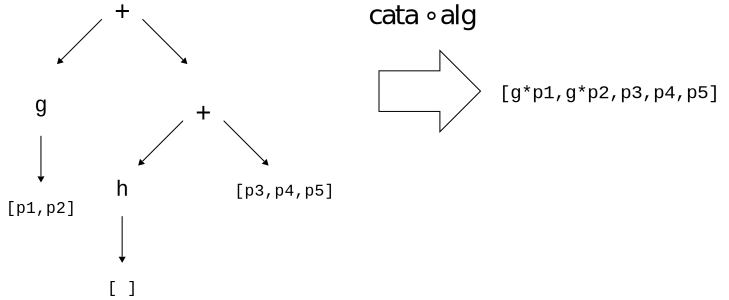
\includegraphics[width=0.7\textwidth]{./figs/flattree.pdf}
    \end{center}
  \end{figure}
\end{frame}

\begin{frame}[fragile]{Data Visualization + Category Theory}
    \begin{center}
        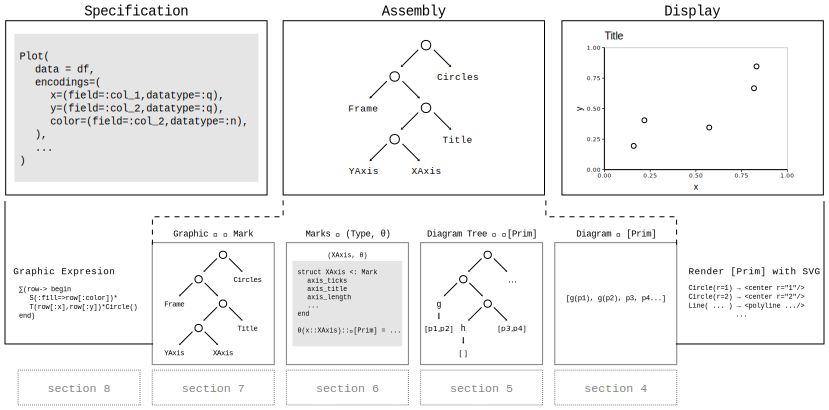
\includegraphics[width=0.9\textwidth]{./figs/pipe.pdf}
    \end{center}
\end{frame}

\begin{frame}[fragile]{Data Visualization + Category Theory}
  The current definitions of marks equate them with primitives. We propose
  a new definition:

  \vspace{3mm}

  Def: A \textbf{Graphical Mark} is a tuple $(A,\theta_A)$, where $A$ is a type and $\theta_A$
  is a function $\theta_A : A \to \mathbb T \text{[Prim]}$.

  \vspace{3mm}

  \begin{minipage}{0.55\textwidth}
  \begin{lstlisting}[language=JuliaLocal, style=julia, texcl=true, escapeinside={(@}{@)}]
struct Face <: Mark
  size::Real
  smile::Real
end

function θ(face::Face)
  eyes = Circle(...) + Circle(...)
  smile = Bezier(...)
  head = Circle(...)

  return head + eyes + smile
end
  \end{lstlisting}
  \end{minipage}
  \hfill
  \begin{minipage}{0.4\textwidth}
    \centering
    
\includegraphics[width=0.8\textwidth]{./figs/face.pdf}
  \end{minipage}

\end{frame}

\begin{frame}[fragile]{Data Visualization + Category Theory}
  We want to be able to define marks using previously defined marks.
  In other words, instead of specifying $\theta_A: A \to \mathbb T [Prim]$,
  we want to define a function $\zeta_A: A \to \mathbb T \text{Mark}$. In other words,
  we want use $\zeta_A$ to infer $\theta_A$.
  \begin{figure}
    \begin{center}
        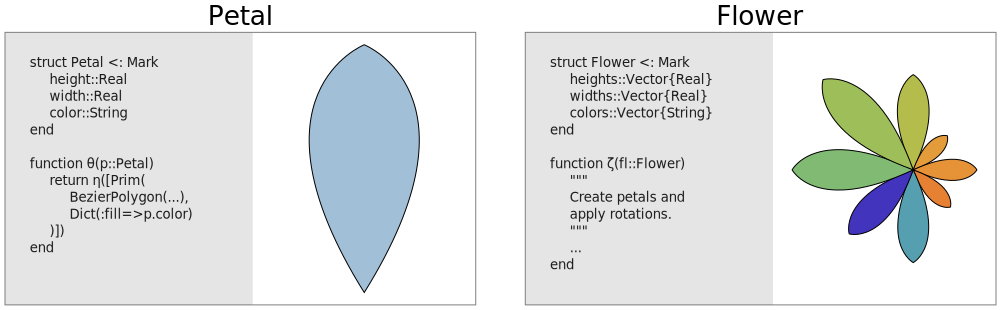
\includegraphics[width=1.0\textwidth]{./figs/petal_flower.pdf}
    \end{center}
  \end{figure}
\end{frame}

\begin{frame}[fragile]{Data Visualization + Category Theory}
  Our $\zeta$ function can be formalized through the use
  of slice categories.

  \vspace{3mm}

  \textbf{Def.} The category of marks $\mathcal M$ is
  a subcategory of  $\textbf{Set}_\mathbb T \slash \text{[Prim]}$.

  \vspace{3mm}

  Assuming this category, a morphism
  $\zeta_A \in \text{Hom}_\mathcal{M}(A, B)$ induces
  $$\theta_A = \theta_{\mathbb T B} \circ \zeta_A = \mu \circ \mathbb T \theta_B \circ \zeta_A$$


  This means that given an existing mark $(B, \theta_b)$, we can
  define a new mark $(A, \theta_A)$ by defining $\zeta_A$ and inferring
  of $\theta_A$.

  \vspace{3mm}

  Programmatically, we can define an abstract type `Mark`, such
  that every subtype of `Mark` has a $theta$ function.
\end{frame}

\begin{frame}[fragile]{Data Visualization + Category Theory}
    \centering
    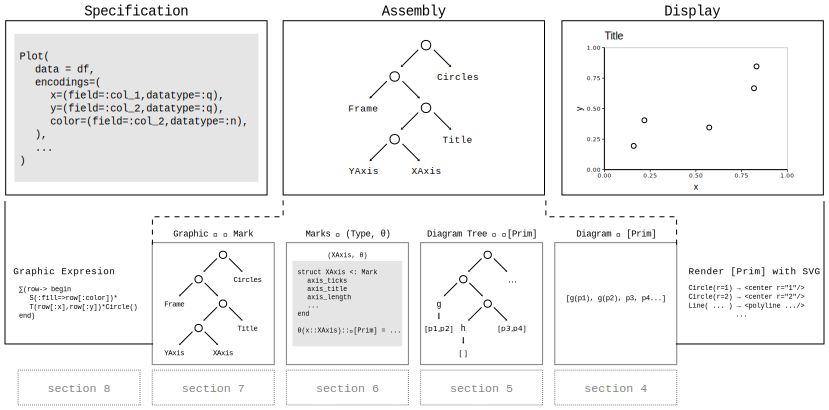
\includegraphics[width=0.9\textwidth]{figs/pipe.pdf}
\end{frame}

\begin{frame}[fragile]{Data Visualization + Category Theory}
  In summary:
  \begin{itemize}
      \item A diagram is a value of [Prim];
      \item A diagram tree is a value of $\mathbb T \text{[Prim]}$;
      \item A mark is a value of type \texttt{A <: Mark} for which $\exists \theta:A \to \mathbb T\text{[Prim]}$;
  \end{itemize}

  \vspace{3mm}
   
   With all these concepts in mind, we can define \textbf{graphic} as a value of $\mathbb T \text{Mark}$,
  i.e. a tree where the leafs contain marks. Since each mark has a $\theta$ function,
  we can turn a $\mathbb T\text{Mark}$ into a $\mathbb T \text{[Prim]}$ using $\mu \circ \mathbb T \theta$.

  \vspace{3mm}

  Note that $\mathbb T \theta: \mathbb T\text{Mark} \to \mathbb T \mathbb T \text{Mark}$ and
  $\mu:\mathbb T \circ \mathbb T \to \mathbb T$.
\end{frame}


\begin{frame}[fragile]{Data Visualization + Category Theory}
  Using $+$ as diagram composition and $*$ to apply transformations,
  we can construct values of $\mathbb T\text{Mark}$ using a notation similar to
  mathematical expressions:
  \begin{figure}
    \begin{center}
        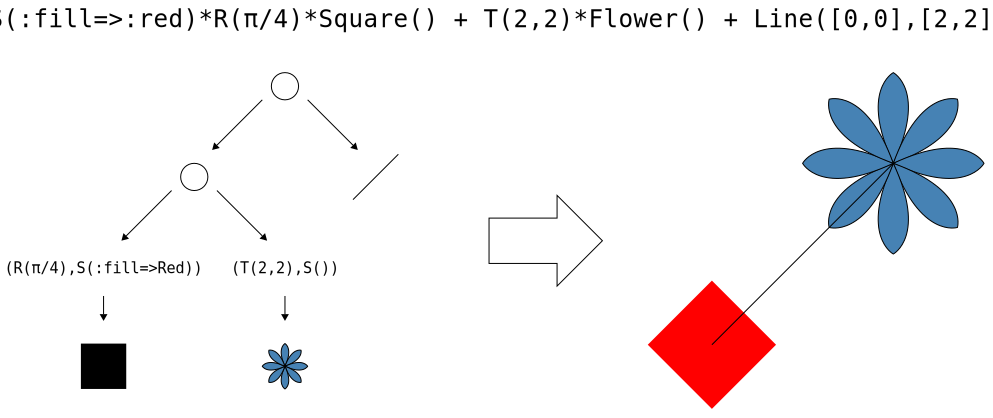
\includegraphics[width=0.8\textwidth]{./figs/graphic.pdf}
    \end{center}
  \end{figure}
\end{frame}

\begin{frame}[fragile]{Data Visualization + Category Theory}
    \centering
    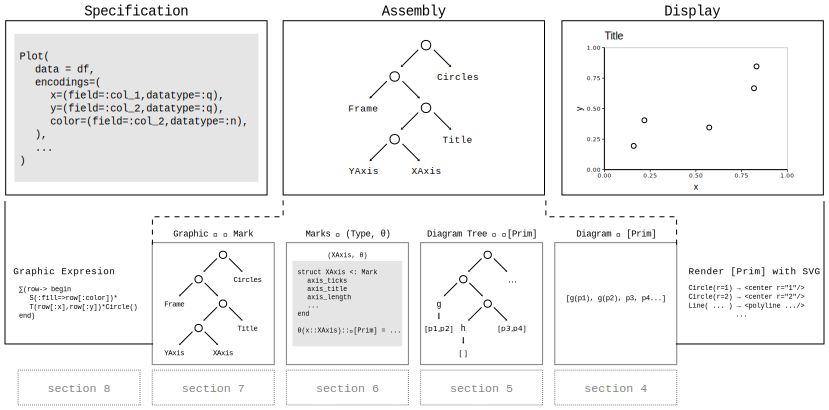
\includegraphics[width=0.9\textwidth]{figs/pipe.pdf}
\end{frame}

\begin{frame}[fragile]{Data Visualization + Category Theory}
    \textbf{Plot Specifications}
    $$\text{Plot} = \text{Guide} + \text{Graphic Expression} \circ \text{Scale(Data, Encodings)}$$
  \begin{figure}
    \begin{center}
        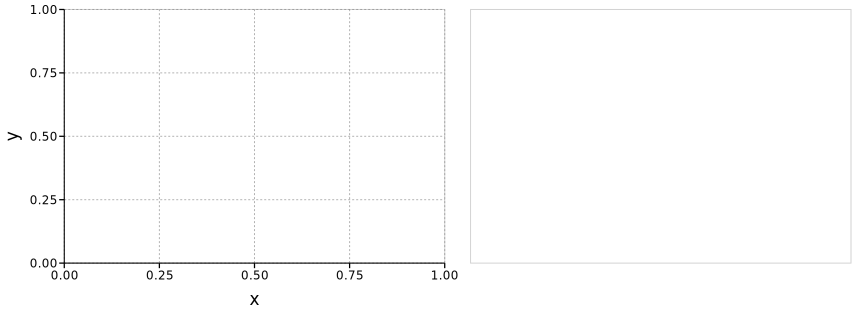
\includegraphics[width=0.8\textwidth]{./figs/frame_graphic.pdf}
    \end{center}
  \end{figure}
\end{frame}

\begin{frame}[fragile]{Data Visualization + Category Theory}
  Guides are the visual aids which
  enable users to decode information regarding the visualization.
  Encodings are dictionaries which describe how to scale
  data attributes, with each encoding having a channel, a field and
  a scale.
  \begin{figure}
    \begin{center}
        
\includegraphics[width=0.8\textwidth]{./figs/scaleddata.pdf}
    \end{center}
  \end{figure}
\end{frame}

\begin{frame}[fragile]{Data Visualization + Category Theory}
  The \textbf{graphic expression} is a function that takes as input
  the scaled data and returns a graphic. It iterates through the data,
  creating several graphical elements, which are then combined together
  to form the graphic. More formally, a graphic expression is a triple
  $(expr,alg,coalg)$, where:
    \begin{align*}
        \sum^{alg}_{coalg}expr \cong \left[
        \begin{array}{@{}c@{}}
            \begin{aligned}
                &expr : D\to \mathbb T \texttt{\{Mark\}} \\
                &alg : [\mathbb T \texttt{\{Mark\}}]\to \mathbb T\texttt{\{Mark\}} \\
                &coalg : D\to \texttt{[}D\texttt{]}
            \end{aligned}
        \end{array}
    \right] 
    \end{align*}
\end{frame}

\begin{frame}[fragile]{Data Visualization + Category Theory}
  The graphic expression is very similar to the split-apply-combine
  pattern. The coalgebra does the splitting, the expression does the
  apply and the algebra does the combine.

  \begin{figure}
    \begin{center}
        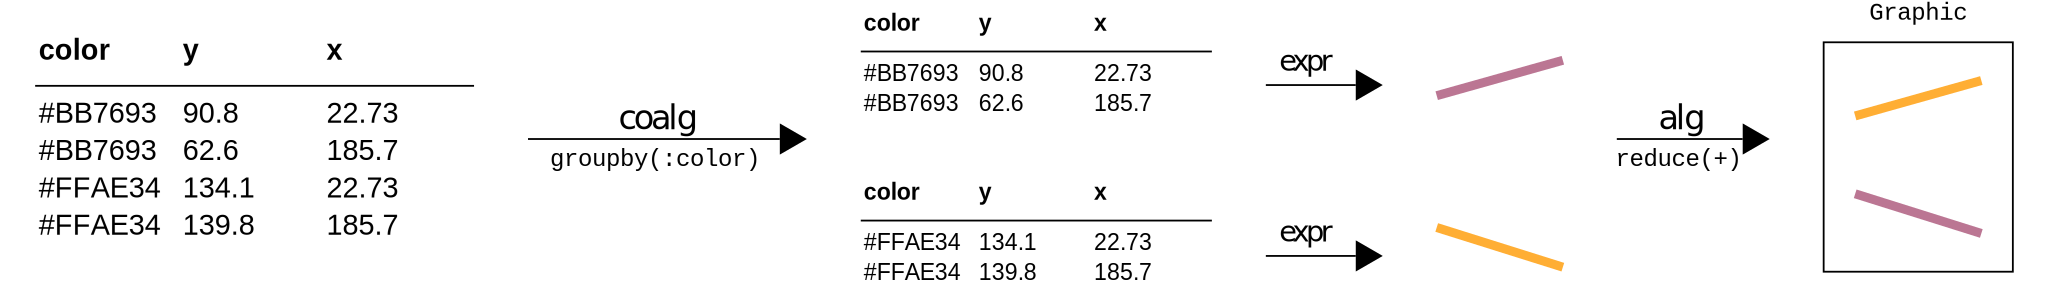
\includegraphics[width=1.0\textwidth]{./figs/graphicexpression.pdf}
    \end{center}
  \end{figure}
\end{frame}


\begin{frame}[fragile]{Data Visualization + Category Theory}
  Here are some examples of graphic expressions:

  $$
  \sum^{+}_{\text{row} \in D} \text{T(row[:x],row[:y]) * Circle(r=row[:size])}
  $$

  \vspace{3mm}

  $$
  \sum^{+}_{\text{gdf} \in D_\text{color}} \text{Line(gdf[:x],gdf[:y],color=gdf[1,:color])}
  $$
\end{frame}

% %------------------------------------------------
% \begin{frame}{References}
%     \footnotesize
%     \bibliography{reference.bib}
%     \bibliographystyle{apalike}
% \end{frame}

%------------------------------------------------

\begin{frame}
    \Huge{\centerline{\textbf{The End}}}
\end{frame}

%----------------------------------------------------------------------------------------

\end{document}
